\documentclass[a4paper,12pt,heading]{ctexbook}

\usepackage{subfiles}
\usepackage{mythesis}

\begin{document}

\subfile{front}

% 目录
%\frontmatter
\tableofcontents

%\pagestyle{main}
% 简介
\subfile{intro}

\subfile{prob}
\section{主要结论}\label{sec:main}
\subsection{初步聚类的正确性}

\subsection{确定性模型}
%We start by defining some key concepts.
We start by defining two concepts adapted from the original proposal of \cite{soltanolkotabi2011geometric}.
\begin{definition}[投影对偶空间]\label{def:proj_dual_direction}
  令 $N$ 为下面对偶问题的最优解
  \begin{align*}
    \max_{N} \; \langle Y, N \rangle - \frac{1}{2\lambda}\| N
    \|_F^2,\quad\text{subject to:}\quad &\|N^T X\|_{2, \infty} \leq 1;
  \end{align*}
  $\mathcal{S}$ 为一个低维子空间。令$ \tilde{N} := \mathbb{P}_{\mathcal{S}} N$,
  对$\tilde{N}$ 进行紧致svd,有
  $$ \tilde{N} = \tilde{U} \Sigma V^T, \quad \tilde{U} \in \mathbb{R}^{d \times r}. $$
  则{\em 投影对偶空间} $\mathcal{U}$ 定义为
  $$\mathcal{U}(Y,X,\mathcal{S},\lambda)\triangleq \spa \{ \tilde{U}_i, i = 1\dots r \}.$$
\end{definition}
 %One way to interpret the optimal solution $N$ is that this is the Euclidean projection of $\lambda x$ to the polytope $\|X^TN\|_{\infty} \leq 1$ and $v$ is the direction of the projection of $N$ to subspace $\cS$.


\begin{definition}[投影子空间的非相干性]\label{def:incoherence}
  对于第$l$个子空间,我们指标集$I$,和其对应的投影对偶空间
  $\mathcal{U}_I^{(\ell)}=\mathcal{U}(X_I^{(\ell)},X_{I^c}^{(\ell)},\mathcal{S}_{\ell},\lambda)$。
  我们称集合 $\mathcal{X}_{\ell}$ 和其他点的不相干度为 $\mu$,如果
  \begin{align*}
    \mu\geq \mu(\mathcal{X}_{\ell}) := &\max_{y\in \mathcal{Y}\setminus \mathcal{Y}_{\ell}}
    \max_{I \in \mathcal{I}(l)} \|\mathbb{P}_{\mathcal{U_I}} y\|_2.
  \end{align*}
\end{definition}
%
%\begin{definition}[Incoherence property]
%There exists small constant $\mu$ such that
%\begin{align*}
%    \mu(S_{\ell}) := &\max_{y\in \mathcal{Y}\setminus \mathcal{Y}_{\ell}}{|\mathbb{P}_{S_{\ell}}(y)|}
%\end{align*}
%where $\mathbb{P}_{S_{\ell}}$ is the projection to subspace $S_{\ell}$.
%\end{definition}

Here, $\mu$ measures the incoherence between corrupted subspace samples $\mathcal{X}_{\ell}$ and clean data points in other subspaces (illustrated in Figure~\ref{fig:SubspaceIncoherence}). As $\|y\|=1$ by the normalization assumption, the range of $\mu$ is $[0,1]$. In case of random subspaces in high dimension, $\mu$ is close to zero. Moreover, as we will see later, for deterministic subspaces and random data points, $\mu$ is proportional to their expected angular distance (measured by cosine of canonical angles).

Definition~\ref{def:proj_dual_direction}~and~\ref{def:incoherence} differ from the \emph{dual direction} and \emph{subspace incoherence property} of \cite{soltanolkotabi2011geometric} in that we require a projection to a particular subspace to cater to the analysis of the noise case. Also, since they reduce to the original definitions when data are noiseless and $\lambda\rightarrow \infty$, these definitions can be considered as a generalization of their original version.

%\begin{figure}
%  \centering
%  % Requires \usepackage{graphicx}
%
%\end{figure}
\begin{figure}
  \centering
  % Requires \usepackage{graphicx}
  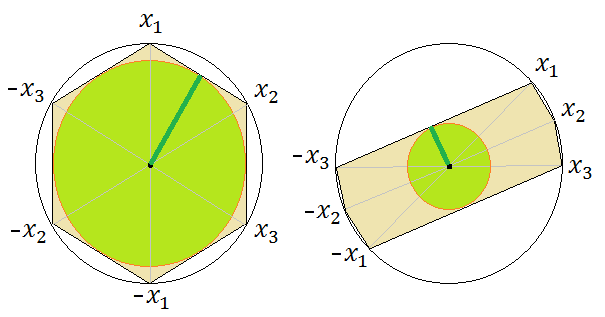
\includegraphics[width=0.7\linewidth]{pics/inradius.png}\\
  \caption{Illustration of inradius and data distribution. The inradius measures how well data points represent a subspace. }\label{fig:inradius}
  \includegraphics[width=0.9\linewidth]{pics/DualDirection.png}\\
  \includegraphics[width=0.9\linewidth]{pics/SubspaceIncoherence.png}
  \caption{Illustrations of the projected dual direction and subspace incoherence property. Jointly, $\left\{x \middle| \max_{i}\big|\langle v_i^{(\ell)},x\rangle\big|\leq \mu\right\}$ defines a polygon in the subspace $\cS_\ell$, and subspace incoherence $\mu$ is given by the smallest such polytope that contains the projections of all external point $y$ into the this subspace.}\label{fig:SubspaceIncoherence}
\end{figure}


%Compare to \citeauthor{soltanolkotabi2011geometric}'s original definition of dual direction and subspace incoherence, we add the projection to a particular subspace, which opens up the possibility for analysis under noise.

\begin{definition}[inradius]
The inradius of a convex body $\mathcal{P}$, denoted by $r(\mathcal{P})$, is defined as the radius of the largest Euclidean ball inscribed in $\mathcal{P}$.
\end{definition}
The inradius of a $\mathcal{Q}_{I^c}^{(\ell)}$ describes the dispersion of the data points. Well-dispersed data lead to larger inradius and skewed/concentrated distribution of data have small inradius. An illustration is given in Figure~\ref{fig:inradius}.


\begin{definition}[Deterministic noise model]
Consider arbitrary additive noise $Z$ to $Y$, each column $z_i$ is bounded by the two quantities below:
\begin{align*}
  \delta:= \max_i\|z_i\|, && \delta_1:=\max_{i,\ell}\|\mathbb{P}_\mathcal{S_{\ell}}z_i\|,
   %&& \delta_2:=\max_{i,\ell}\|\mathbb{P}_\mathcal{S_{\ell}^{\perp}}z_i\|.
\end{align*}
\end{definition}
As we assume the uncorrupted data point $y$ has unit norm, $\delta$ essentially describes the amount of allowable relative error.


\begin{theorem}\label{thm:thm_general}
Under the deterministic noise model, compactly denote
\begin{align*}
\mu_{\ell}:=\mu(\mathcal{X}_{\ell}),&& r_{\ell}:=\min_{\{i: x_i\in \mathcal{X}_{\ell}\}}r(\mathcal{Q}^{(\ell)}_{I^c}),&&
   r:=\min_{\ell=1,...,L} r_{\ell}.
\end{align*}
If $\mu_{\ell}< r_{\ell}$ for each $\ell = 1,...,L$, furthermore
$$ \delta\leq \min_{\ell=1,...,L}\frac{r(r_{\ell}-\mu_{\ell})}{2+7r_{\ell}} $$
then LASSO subspace detection property holds for all weighting parameter $\lambda$ in the range
\begin{equation*}
\frac{1}{r - 2\delta-\delta^2}<
        \lambda<\min_{\ell=1,..,L}\left\{\frac{r_{\ell}-\mu_{\ell}-2\delta_1}{\delta(1+\delta)(2+r_{\ell}-\delta_1)}\right\}
\end{equation*}
%\begin{equation*}
%\left\{\begin{aligned}
%  \lambda&>\frac{1}{(r-\delta_1)(1-3\delta) - 3\delta-2\delta^2}\\
%  \lambda&<\min_{\ell=1,..,L}\left\{\frac{r_{\ell}-\mu_{\ell}-2\delta_1}{\delta(1+\delta)(3+2r_{\ell}-2\delta_1)}\right\}\vee\frac{2r}{\delta^2(r+1)}.
%\end{aligned}\right.
%\end{equation*}
which is guaranteed to be non-empty.
\end{theorem}
We now offer some discussions of the theorem and the proof will be given in  Section~\ref{chp:proof_deterministic}.
%\begin{theorem}\label{thm:thm_general}
%Under deterministic noise model, compactly denote
%\begin{align*}
%  \rho:=2\lambda\delta(1+\delta),&&r:=\min_{\ell=1,...,k} \min_{\{i: x_i\in \mathcal{X}_{\ell}\}}r(\mathcal{Q}^{(\ell)}_{I^c}),&&\mu=\max_{\ell=1,...,k} \mu(\mathcal{X}_{\ell}).
%\end{align*}
%If $\mu< r$, furthermore
%$$ \delta\leq\frac{r(r-\mu)}{3r^2+7r+2}, $$
%then for each $\ell=1,...,k$, the solution $(c_i,e_i)$ to \eqref{eq:Opt_original} for $x_i\in \mathcal{X}_{\ell}$ satisfies:
%(1)$c_i \neq 0$,
%(2)support of $c_i$ corresponds to only columns of $X$ belonging to $\mathcal{X}_{\ell}$,
%for any weighting parameter $\lambda$ in the non-empty range:
%$$
%  \frac{1}{(r-\delta_1)(1-3\delta) - 2\delta}< \lambda < \min\left\{\frac{r-\mu-2\delta_1}{2\delta(1+\delta)(r-\delta_1+1)},\frac{2r}{\delta^2(r+1)}\right\}.
%$$
%\end{theorem}



%\begin{remark}[Noiseless case]
\paragraph{Noiseless case.} When $\delta=0$,  i.e., there is no noise, the condition reduces to $\mu_{\ell}< r_{\ell}$, which coincides with the result in \cite{soltanolkotabi2011geometric}. The exact LP formulation~\eqref{eq:SSC} is equivalent to $\lambda \rightarrow \infty$. Our result implies that unconstrained LASSO formulation \eqref{eq:Lasso} works for any $\lambda>\frac{1}{r}$. %{\color{red}[The last sentence is broken.]}
%\end{remark}

%\begin{remark}[Signal-to-Noise Ratio]
\paragraph{Signal-to-Noise Ratio.} Condition $\delta\leq\frac{r(r-\mu)}{2+7r}$ can be interpreted as the breaking point under increasing magnitude of attack. This suggests that SSC by \eqref{eq:Lasso} is provably robust to arbitrary noise having signal-to-noise ratio~(SNR) greater than $\Theta\big(\frac{1}{r(r-\mu)}\big)$. (Notice that $0<r<1$, and hence $7r+2 =\Theta(1)$.)
%\end{remark}

\paragraph{Tuning parameter $\lambda$.} The range of the parameter $\lambda$ in the theorem depends on unknown parameters $\mu$, $r$ and $\delta$, and therefore cannot be used in practice to choose the parameter in practice. It does however justify that when $\delta$ is small, the range of $\lambda$ that Lasso-SSC works is large, therefore not hard to tune. In practice, we do not need to know $\lambda$ in prior. One approach is to trace the Lasso path \cite{tibshirani2013lasso} until we have about $k$ non-zero entries in the coefficient vector. If we would like to use a single $\lambda$ for all columns, a good point to start is to take $\lambda$ to be in the order of $O\big(\frac{1}{\min_j \max_{i\neq j}|x_i^Tx_j|}\big)$, this ensures the solution to be at least non-trivial.


\paragraph{Agnostic subspace clustering.}
The robustness to deterministic error is important, since in practice the union-of-subspace structures are usually only good approximations. If each subspace has decaying singular values (e.g., motion segmentation, face clustering \cite{elhamifar2012ssc_journal} and hybrid system identification\cite{vidal2003algebraic}), the deterministic guarantee allows for the flexibility in choosing the cut-off points, e.g., take 90\% of the energy as signal and treat the remaining spectrum as noise. If one keeps a smaller number of singular values ( a smaller subspace dimension), the inradius will likely to be larger \footnote{A formal relationship between inradius and smallest singular value is described in \cite{wang2013provable}.}, although the noise level also increases. It is  possible that the conditions in Theorem~\ref{thm:thm_general} are satisfied for some decomposition (e.g., those with a large spectral gap) but not others. The nice thing is that this is not a tuning parameter, but rather a theoretical property that remains agnostic to the users. In fact, the algorithm will be provably effective as long as the conditions are satisfied for any signal noise decomposition (not restricted to rank-projection). None of these is possible if distributional assumptions are made to either the data or the noise.








%\begin{figure}
%  \centering
%  \includegraphics[width=0.8\textwidth]{pics/Noiseless_vs_Noisy.png}\\
%   \caption{Geometric interpretation and comparison of the noiseless SSC (\textbf{Left}) and noisy LASSO-SSC (\textbf{Right}).}
%   \label{fig:geom_interpretation}
%\end{figure}



%\begin{figure}
%  \centering
%  \includegraphics[width=7cm]{pics/NoiselessGuarantee.png}\\
%   \caption{Noiseless SSC: Theorem~2.5 of \cite{soltanolkotabi2011geometric} suggests that the projection of external data points must fall inside the solid blue polygon, which is the intersection of halfspaces defined by dual directions (blue dots) that are tangent planes of the red inscribing sphere.}
%   \label{fig.noiseless_guarantee}
%\end{figure}
%\begin{figure}
%  \centering
%  \includegraphics[width=7cm]{pics/NoisyGuarantee.png}\\
%  \caption{Noisy LASSO-SSC: The guarantee of Theorem~\ref{thm:thm_general} means that the whole red sphere of each external data points must fall inside the dashed red polygon, which is smaller than the blue polygon by a factor related to the noise level. } \label{fig.noisy_guarantee}
%\end{figure}

\subsection{Randomized models}
We  further analyze three randomized models with increasing level of randomness.
\begin{description}
  \item[$\bullet$ Determinitic+Random Noise.] Subspaces and samples in subspace are arbitrary; the noise obeys the Random Noise model (Definition~\ref{def:Random_noise_model}).
  \item[$\bullet$ Semi-random+Random Noise.] Subspace is deterministic, but samples in each subspace are drawn iid uniformly from the intersection of the unit sphere and the subspace; the noise obeys the Random Noise model.
  \item[$\bullet$ Fully random.] Both subspace and samples are drawn uniformly at random from their respective domains; the noise is iid Gaussian.%\footnote{It is straightforward to state the model for Definition~\ref{def:Random_noise_model}. We choose Gaussian as an illustration.}.
\end{description}

\begin{definition}[Random noise model]\label{def:Random_noise_model}
Our random noise model is defined to be any additive $Z$ that is (1) columnwise iid; (2) spherical symmetric;  and (3) $\|z_i\|\leq \delta$ for all $i=1,...,N$ with probability at least $1-1/N$.
\end{definition}
%\begin{example}[Gaussian noise]
$$\P\left(\delta:=\max_i\|z_i\| > \sqrt{1+\frac{6\log N}{n}}\sigma\right) \leq C/N^2.$$
%\end{example}

\begin{theorem}[Deterministic+Random Noise]\label{thm:thm_random_noise}
 Under random noise model, compactly denote $r_{\ell}$, $r$ and $\mu_{\ell}$ as in Theorem~\ref{thm:thm_general}, furthermore let
$$\epsilon := \sqrt{\frac{6\log N}{n-\max_{\ell}{d_{\ell}}}}\leq \sqrt{\frac{C\log(N)}{n}}.$$
 %$$\epsilon := \sqrt{\frac{6\log N+2\log \max_{\ell}{d_{\ell}}}{n-\max_{\ell}{d_{\ell}}}}\leq \sqrt{\frac{C\log(N)}{n}} .$$
 If $\mu_{\ell}<r_{\ell}$ for all $\ell = 1,...,k$,
 \begin{align*}
 \epsilon\delta<\min_{\ell=1,...,L}\frac{r_{\ell}-\mu_{\ell}}{2\sqrt{d_{\ell}}+2}, &&\text{and}&& \epsilon\delta(1+\delta) < \min_{\ell=1,...,L}\frac{r(r_\ell-\mu_\ell)}{4r_\ell+6},
\end{align*}
 %$$\delta<\min_{\ell=1,...,L}\frac{r_{\ell}-\mu_{\ell}}{2r_{\ell}+4},$$
then with probability at least $1-9/N$, LASSO subspace detection property holds for all weighting parameter $\lambda$ in the range
\begin{equation}\label{eq:thm_rand_noise_lambda_range}
\frac{1}{r- 2\epsilon \delta-\epsilon\delta^2}<
        \lambda<\min_{\ell=1,...,L}\left\{\frac{r_{\ell}-\mu_{\ell}-\delta\epsilon - \delta \sqrt{d_{\ell}} \epsilon}{\epsilon\delta(1+\delta)(3+r_{\ell}-\delta\sqrt{d_{\ell}}\epsilon)}\right\}
%\frac{1}{(r-\delta\epsilon)(1-2\delta) - 2\delta-\delta^2}<
%        \lambda<\min_{\ell=1,...,L}\left\{\frac{r_{\ell}-\mu_{\ell}-2\delta\epsilon}{\epsilon\delta(1+\delta)(2+r_{\ell}-\delta\epsilon)}\right\}
\end{equation}
which is guaranteed to be non-empty.
\end{theorem}
\paragraph{Low SnR paradigm.} Compared to Theorem~\ref{thm:thm_general}, Theorem~\ref{thm:thm_random_noise} considers a more benign noise which leads to a stronger result. In particular, without assuming any statistical model on how data are generated, we show that Lasso-SSC is able to tolerate noise of level $O\left((\frac{n}{\log N})^{1/4}(r(r_\ell-\mu_\ell))^{1/2}\right)$ or $O\left((\frac{n}{d\log N})^{1/2}(r_\ell-\mu_\ell)\right)$ (whichever is smaller). This extends SSC's guarantee with deterministic data to cases where the noise can be significantly larger than the signal. In fact, the SnR can go to $0$ as the ambient dimension gets large.

On the other hand, Theorem~\ref{thm:thm_random_noise} shows that Lasso-SSC is able to tolerate a constant level of noise when the geometric gap $r_\ell-\mu_\ell$ is as small as $O(\sqrt{d/n})$. This is arguably near-optimal (when $d$ is small) as the projection of a constant-level random noise into a $d$-dimensional subspace has an expected magnitude of the same order, which could easily close up the small geometric gap for some non-trivial probability if the noise is much larger.

%We note that the projection of the random noise into the subspace ($\delta_1$) has the magnitude of the same order $O(\sqrt{d/n})$. {\color{red}[Not sure what the last sentence means.]} % I was intending to argue that this is big enough to distort everything in the subspace almost arbitrarily.


\paragraph{Margin of error.}
Since the bound depends critically on $(r_\ell-\mu_\ell)$~--~the difference of inradius and incoherence~--~which is the geometric gap that appears in the noiseless guarantee of \cite{soltanolkotabi2011geometric}. We will henceforth call this gap the \emph{margin of error}.

We now analyze this margin of error under different generative models. We
start from the semi-random model, where the distance between two subspaces is measured as follows.
\begin{definition}\label{def:subspace_affinity}
The {\em affinity} between two subspaces is defined by:
$$ \mathrm{aff}(\mathcal{S}_k,\mathcal{S}_{\ell}) = \sqrt{\cos^2{\theta^{(1)}_{k\ell }}+...+\cos^2{\theta^{(\min(d_k,d_{\ell}))}_{k\ell}}},$$
where $\theta_{k\ell}^{(i)}$ is the $i^{th}$ canonical angle between the two subspaces. Let $U_{k}$ and $U_{\ell}$ be a set of orthonormal bases of each subspace, then $\mathrm{aff}(\mathcal{S}_k,\mathcal{S}_{\ell})=\|U_{k}^TU_{\ell}\|_F$.
\end{definition}
When data points are randomly sampled from each subspace, the geometric entity $\mu(\mathcal{X}_{\ell})$ can be expressed using this (more intuitive) subspace affinity, which leads to the following theorem.


\begin{theorem}[Semi-random model+random noise]\label{thm:semirandom}
Under the semi-random model with random noise, there exists a non-empty range of $\lambda$ such that LASSO subspace detection property holds with probability $1- \frac{9}{N} - \frac{1}{L^2}\sum_{\ell\neq \ell^\prime}\frac{1}{(N_{\ell}+1)N_{\ell^\prime}} e^{-\frac{t}{4}} -6\sum_{\ell=1}^L (e^{\gamma_1 (n-d_\ell)}+e^{\gamma_2 d_\ell}+e^{-\sqrt{N_{\ell}d_{\ell}}})$ as long as the noise level obeys
\begin{align*}
 \delta(1+\delta) \leq& \max_{\ell,\ell'}\sqrt{\frac{n-d}{6\log N}} \frac{\sqrt{\log \kappa}}{40K_2\sqrt{dd_\ell}}\left(1- \frac{K_1K_2 \mathrm{aff}(\mathcal{S}_{\ell},\mathcal{S}_{\ell^\prime})}{\sqrt{ d_{\ell^\prime}}} \right),
\end{align*}
where $K_1:= (t \log  [(N_{\ell}+1)N_{\ell^\prime}] + \log L)$, $K_2 := 4\sqrt{\frac{1}{\log\kappa_\ell}}$, $\kappa_\ell := N_{\ell}/d_{\ell}$, $\frac{\log\kappa}{d} :=\min_{\ell} \frac{\log\kappa_\ell}{d_\ell}$, and
$\gamma_1,\gamma_2$ are absolute constants.
\end{theorem}
The proof is essentially substituting the incoherence and inradius parameters in Theorem~\ref{thm:thm_random_noise} with meaningful bounds, so Thereom~\ref{thm:semirandom} can be regarded as a corollary of Theorem~\ref{thm:thm_random_noise}.

\paragraph{Overlapping subspaces.}
Similar to the results in \cite{soltanolkotabi2011geometric}, Theorem~\ref{thm:semirandom} demonstrates that LASSO-SSC can handle overlapping subspaces with noisy samples. By Definition~\ref{def:subspace_affinity}, $\mathrm{aff}(\mathcal{S}_k,\mathcal{S}_{\ell})$ can be small even if $\mathcal{S}_k$ and $\mathcal{S}_{\ell}$ share a basis.

\paragraph{Comparison to \cite{soltanolkotabi2013robust}.}
In the high dimensional setting when $n\gg d$, our result is able to handle the low SnR regime when $\delta = \Theta(n^{1/4}/d^{1/2})$, while \cite{soltanolkotabi2013robust} needs $\delta$ to be bounded by a small constant.

In the case when $d$ is a constant fraction of $n$, however, our bound is worse by a factor of $\sqrt{d}$. \cite{soltanolkotabi2013robust} is still able to handle a small constant noise while we needs $\delta < O(\frac{1}{\sqrt{d}})$. The suboptimal bound might be due to the fact that we are simply developing the theorem for the semirandom model as a corollary of Theorem~\ref{thm:thm_random_noise} and haven not fully exploit the structure of the semi-random model in the proof.

%Lastly, our result does not invoke the Restricted Isometry Property (RIP) bound at any point of the analysis therefore does not have any restrictions on the subspace dimension.  %The point is made more explicitly in the fully random model in Theorem~\ref{thm:fullrandom2}.
%In fact, if we are willing to assume $d>\log N$, we can apply the intermediate results in the proof of \cite{soltanolkotabi2013robust} to further improve the bound to handle $\delta = \Theta((n/d)^{1/4})$ (see appendix for details), this matches the best known results for noisy subspace clustering using TSC \cite{heckel2013robust}.


We now turn to the fully random case.
\begin{theorem}[Fully random model]\label{thm:fullrandom}
Suppose there are $L$ subspaces each with dimension $d$, chosen independently and uniformly at random. For each subspace, $\kappa d+1$ points are chosen independently and uniformly from the unit sphere inside each subspace. Each measurement is corrupted by iid Gaussian noise $\sim N(0,\sigma^2/n)$. Furthermore, if
\begin{align*}
  d < \frac{c(\kappa)^2\log\kappa}{24\log N} n, &&\text{and} && \sigma(1+\sigma) < \frac{c(\kappa)^2\log \kappa  }{20}\frac{\sqrt{n} }{d},
\end{align*}
then with probability at least $1-\frac{10}{N}-Ne^{-\sqrt{\kappa}d}$, the LASSO subspace detection property holds for any $\lambda$ in the range
\begin{equation}\label{eq:thm_rand_lambda_range}
  \frac{C_1\sqrt{d}}{c(\kappa)\sqrt{\log \kappa}}<\lambda <  \frac{C_2c(\kappa)\sqrt{n\log\kappa}}{\sigma\sqrt{d\log N}},
\end{equation}
which is guaranteed to be non-empty. Here, $C_1,C_2$ are absolute constants.
\end{theorem}
The results under this simple model are very interpretable. It
 provides intuitive guideline in how robustness of Lasso-SSC change with respect to the various parameters of the data.
 One one hand, it is sensitive to the dimension of each subspace $d$, since the $\sigma \leq \tilde{\Theta}(\frac{n^{1/4}}{\sqrt{d}})$. This dependence on subspace dimension $d$ is not a critical limitation as most interesting applications indeed have very low subspace-dimension, as summarized in Table~\ref{tab:low_rank}.
On the other hand, the dependence on the number of subspaces $L$ (in both $\log\kappa$ and $\log N$ since $N=L(\kappa d+1)$) is only logarithmic.  This suggests that SSC is robust even when there are many clusters, and $Ld\gg n$.

% such as subspace dimension $d$ and number of subspaces $L$ in the simplistic setting.



%
%\begin{remark}[Trade-off between $d$ and the margin of error]\label{rmk:tradeoff_large_d}
%Theorem~\ref{thm:fullrandom}  extends our results to the paradigm where the subspace dimension grows  linearly with the ambient dimension. Interestingly, it shows that the margin of error scales $\tilde{\Theta}(\sqrt{1/d})$, implying a relationship between $d$ and robustness to noise. Fortunately,  most interesting applications indeed have very low subspace-rank, as summarized in Table~\ref{tab:low_rank}.
%\end{remark}



\begin{table}
  \centering
 \begin{tabular}{|p{0.6\linewidth}|c|}
   \hline
   % after \\: \hline or \cline{col1-col2} \cline{col3-col4} ...
   \textbf{Application} & \textbf{Cluster rank}\\
   \hline
   3D motion segmentation \cite{costeira1998motion_seg} & $\mathrm{rank}=4$ \\\hline
   Face clustering (with shadow) \cite{basri2003lambertianface} & $\mathrm{rank}=9$ \\\hline
   Diffuse photometric face \cite{zhou2007PhotometricFace}& $\mathrm{rank}=3$ \\\hline
   Network topology discovery \cite{eriksson2011high_rankMC} & $\mathrm{rank}=2$ \\\hline
   Hand writing digits \cite{hastie1998MNIST}&  $\mathrm{rank}=12$\\\hline
   Social graph clustering \cite{xu2011graphclustering}& $\mathrm{rank}=1$ \\
   \hline
 \end{tabular}
  \caption{Rank of real subspace clustering problems}\label{tab:low_rank}
\end{table}

%\begin{remark}[Robustness in the many-cluster setting]\label{rmk:large_num_subspace}
%Another interesting observation is that the margin of error scales logarithmically with respect to $L$, the number of clusters (in both $\log\kappa$ and $\log N$ since $N=L(\kappa d+1)$). This suggests that SSC is robust even if there are many clusters, and $Ld\gg n$.
%\end{remark}



%\noindent\textbf{The guarantee in Theorem~\ref{thm:thm_general}:}
\subsection{Geometric interpretations}%  of Theorem~\ref{thm:thm_general}}
A geometric illustration of the condition in Theorem~\ref{thm:thm_general} is given in Figure~\ref{fig:geom_interpretation} in comparison to the geometric separation condition in the noiseless case.

\begin{figure}
        \centering
        \begin{subfigure}[t]{0.4\textwidth}
          \centering
              \includegraphics[width=\textwidth]{pics/NoiselessGuarantee.png}\\
               \caption{Noiseless SSC}
               \label{fig.noiseless_guarantee}
        \end{subfigure}%
        ~ %add desired spacing between images, e. g. ~, \quad, \qquad etc.
          %(or a blank line to force the subfigure onto a new line)
        \begin{subfigure}[t]{0.4\textwidth}
              \centering
              \includegraphics[width=\textwidth]{pics/NoisyGuarantee.png}\\
              \caption{Noisy LASSO-SSC} \label{fig.noisy_guarantee}
        \end{subfigure}
   \caption{Geometric interpretation and comparison of the noiseless SSC (\textbf{Left}) and noisy LASSO-SSC (\textbf{Right}).
   %On the \textbf{left}, Theorem~2.5 of \cite{soltanolkotabi2011geometric} suggests that the projection of external data points must fall inside the solid blue polygon, which is the intersection of halfspaces defined by dual directions (blue dots) that are tangent planes of the red inscribing sphere. On the \textbf{right}, the guarantee of Theorem~\ref{thm:thm_general} means that the whole red sphere of each external data points must fall inside the dashed red polygon, which is smaller than the blue polygon by a factor related to the noise level.
   }
   \label{fig:geom_interpretation}
\end{figure}

The left pane depicts the separation condition $\mu_\ell \leq r_\ell$ in Theorem~2.5 of \cite{soltanolkotabi2011geometric}. The blue polygon represents the the intersection of halfspaces defined with dual directions that are also the tangent to the red inscribing sphere. More precisely, this is $\left\{x\in \cS_\ell \middle| \big|\langle v_i^{\ell}, x\rangle\big| \leq r_\ell\right\}$. From our illustration of $\mu$ in Figure~\ref{fig:SubspaceIncoherence}, we can easily tell that $\mu_\ell\leq r_\ell$ if and only if the projection of external data points fall inside this solid blue polygon. We call this solid blue polygon the successful region.

The right pane illustrates our guarantee of Theorem~\ref{thm:thm_general} under bounded deterministic noise. The successful condition requires that the whole red ball (analogous to uncertainty set in Robust Optimization \cite{ben1998robust,bertsimas2004price}) around each external data point to fall inside the dashed red polygon, which is smaller than the blue polygon by a factor related to the noise level and the inradius.

The successful region is affected by the noise because the design matrix is also arbitrarily perturbed and the dual solution is no longer within each subspace $\cS_\ell$. Specifically, as will become clear in the proof, the key of showing SEP boils down to proving
$
\langle N_i^{(\ell)}, x_j\rangle < 1
$
for all pairs of $(N_i^{(\ell)}, x_j)$ where
$$ N_i^{(\ell)}=\arg\max_{N} \langle N, x_i^{(\ell)}\rangle  -\frac{1}{2\lambda}\|N\|^2 \text{ s.t. }  \|N^TX_{I^c}^{(\ell)} \|_\infty \leq 1,$$
and $x_j$ is any point from another subspace. In the noiseless case we can always take $N_i^{(\ell)}\in\cS_\ell$ and $\langle N_i^{(\ell)}, x_j\rangle \leq \frac{\mu_\ell}{r_\ell}$. For noisy data and Lasso-SSC, we can no longer do that. In fact, for any fixed $\lambda$, the dual solution will be uniquely determined by a projection of $\lambda x_i^{(\ell)}$ on to the feasible region $\|N^TX_{I^c}^{(\ell)} \|_\infty \leq 1$ (see the first pane of Figure~\ref{fig:SubspaceIncoherence}). The absolute value of the inner product $\langle N_i^{(\ell)}, x_j\rangle$ will depend on the magnitude of the dual solution, especially its component perpendicular to the current subspace. Indeed by carefully choosing the error, we can make $\mathbb{P}_{\cS_\ell^{\perp}}N$ very correlated with some external data point $x_j$.

%This is why we need to shrink the size of the successful region to account for the worst case.

To illustrate this further, we plot the shape of this feasible region in 3D (see Figure~\ref{fig.convex_hull_n_polar}(b)). From the feasible region alone, it seems that the magnitude of dual variable can potentially be quite large. Luckily, the quadratic penalty in the objective function allows us to exploit the optimality of the solution $N$ and bound the ``out-of-subspace'' component of $N$, which results in a much smaller region where the solution can potentially be (given in Figure~\ref{fig.convex_hull_n_polar}(c)). The region for the ``in-subspace'' component is also smaller as is shown in Figure~\ref{fig.ProjPolar}. A more detailed argument of this is given in Section~\ref{sec:dual_separation} of the proof.

\begin{figure}
  \centering
%  % Requires \usepackage{graphicx}
%  \includegraphics[width=0.6\linewidth]{pics/CandesDualDirection.png}\\
%  \caption{An illustration of dual direction from \cite{soltanolkotabi2011geometric}.}\label{fig.candes_dual_direction}
    \includegraphics[width=0.7\linewidth]{pics/conv_hull_n_polarset2.png}\\
  \caption{Illustration of \textbf{(a)} the convex hull of noisy data points, \textbf{(b)} its polar set and \textbf{(c)} the intersection of polar set and $\|N_{\parallel}\|$ bound. The polar set (b) defines the feasible region of \eqref{eq:dual_fictitious2}. It is clear that $N_{\parallel}$ can take very large value in (b) if we only consider feasibility. By considering optimality, we know the optimal $N$ must be inside the region in (c).} \label{fig.convex_hull_n_polar}
    \includegraphics[width=0.6\linewidth]{pics/Projected_polarset_cmp1.png}\\
  \caption{The projection of the polar set (the green area) in comparison to the projection of the polar set with $\|N_{\parallel}\|$ bound (the blue polygon). It is clear that the latter is much smaller.}\label{fig.ProjPolar}
\end{figure}

Admittedly, the geometric interpretation under noise is slightly messier than the noiseless case, but it is clear that the largest deterministic noise Lasso-SSC can tolerate must be smaller than geometric gap $r_\ell-\mu_\ell$. Theorem~\ref{thm:thm_general} show that a sufficient condition is $\delta \leq O(r(r_\ell-\mu_\ell))$. It remains unclear whether this gap can be closed without additional assumptions.

%\subsection{Geometric interpretation of Theorem~\ref{thm:thm_random_noise}}

Finally, we note that for the random noise model in Theorem~\ref{thm:thm_random_noise}, the geometric interpretation is similar, except that the impact of the noise is weakened. Thanks to the randomness and the corresponding concentration of measure, we may bound the reduction of the successful region with a much smaller value comparing to the adversarial noise case.

%Algebraically, this is made clear by the \emph{randomized dual separation condition} (see \eqref{eq:dual_sep_random} in Lemma~\ref{lemma:dual_sep_random}). From the robust optimization perspective, this is equivalent to reducing the size of the uncertainty set by leaving the bulk unlikely region of the uncertainty set unconstrained. In other word, the size of the red ball in Figure~\ref{fig:geom_interpretation} is much smaller in the randomized case.








\subfile{greedy}
\subfile{multi}
\subfile{exper}
\begin{thebibliography}{47}
    \providecommand{\natexlab}[1]{#1}
    \providecommand{\url}[1]{\texttt{#1}}
    \expandafter\ifx\csname urlstyle\endcsname\relax
    \providecommand{\doi}[1]{doi: #1}\else
    \providecommand{\doi}{doi: \begingroup \urlstyle{rm}\Url}\fi

    \bibitem[Ball(1997)]{ball1997intro_convex_geometry}
    K.~Ball.
    \newblock An elementary introduction to modern convex geometry.
    \newblock \emph{Flavors of geometry}, 31:\penalty0 1--58, 1997.

    \bibitem[Basri and Jacobs(2003)]{basri2003lambertianface}
    R.~Basri and D.W. Jacobs.
    \newblock Lambertian reflectance and linear subspaces.
    \newblock \emph{Pattern Analysis and Machine Intelligence, IEEE Transactions
    on}, 25\penalty0 (2):\penalty0 218--233, 2003.

    \bibitem[Ben-Tal and Nemirovski(1998)]{ben1998robust}
    A.~Ben-Tal and A.~Nemirovski.
    \newblock Robust convex optimization.
    \newblock \emph{Mathematics of Operations Research}, 23\penalty0 (4):\penalty0
    769--805, 1998.

    \bibitem[Bertsimas and Sim(2004)]{bertsimas2004price}
    D.~Bertsimas and M.~Sim.
    \newblock The price of robustness.
    \newblock \emph{Operations research}, 52\penalty0 (1):\penalty0 35--53, 2004.

    \bibitem[Boyd et~al.(2011)Boyd, Parikh, Chu, Peleato, and
    Eckstein]{boyd2011admm}
    S.~Boyd, N.~Parikh, E.~Chu, B.~Peleato, and J.~Eckstein.
    \newblock Distributed optimization and statistical learning via the alternating
    direction method of multipliers.
    \newblock \emph{Foundations and Trends{\textregistered} in Machine Learning},
    3\penalty0 (1):\penalty0 1--122, 2011.

    \bibitem[Bradley and Mangasarian(2000)]{bradley2000k-plane}
    P.S. Bradley and O.L. Mangasarian.
    \newblock k-plane clustering.
    \newblock \emph{Journal of Global Optimization}, 16\penalty0 (1):\penalty0
    23--32, 2000.

    \bibitem[Brandenberg et~al.(2004)Brandenberg, Dattasharma, Gritzmann, and
    Larman]{brandenberg2004isoradial}
    Ren{\'e} Brandenberg, Abhi Dattasharma, Peter Gritzmann, and David Larman.
    \newblock Isoradial bodies.
    \newblock \emph{Discrete \& Computational Geometry}, 32\penalty0 (4):\penalty0
    447--457, 2004.

    \bibitem[Cand{\`e}s(2008)]{candes2008RIP}
    E.J. Cand{\`e}s.
    \newblock The restricted isometry property and its implications for compressed
    sensing.
    \newblock \emph{Comptes Rendus Mathematique}, 346\penalty0 (9):\penalty0
    589--592, 2008.

    \bibitem[Chen and Lerman(2009)]{chen2009spectral}
    G.~Chen and G.~Lerman.
    \newblock Spectral curvature clustering (scc).
    \newblock \emph{International Journal of Computer Vision}, 81\penalty0
    (3):\penalty0 317--330, 2009.

    \bibitem[Costeira and Kanade(2000)]{costeira2000multibody_factorization}
    Joao Costeira and Takeo Kanade.
    \newblock \emph{A multi-body factorization method for motion analysis}.
    \newblock Springer, 2000.

    \bibitem[Costeira and Kanade(1998)]{costeira1998motion_seg}
    J.P. Costeira and T.~Kanade.
    \newblock A multibody factorization method for independently moving objects.
    \newblock \emph{International Journal of Computer Vision}, 29\penalty0
    (3):\penalty0 159--179, 1998.

    \bibitem[Dasgupta and Gupta(2002)]{dasgupta2002xi_square_concentration}
    S.~Dasgupta and A.~Gupta.
    \newblock An elementary proof of a theorem of johnson and lindenstrauss.
    \newblock \emph{Random Structures \& Algorithms}, 22\penalty0 (1):\penalty0
    60--65, 2002.

    \bibitem[Donoho(1995)]{donoho1995noising}
    D.L. Donoho.
    \newblock De-noising by soft-thresholding.
    \newblock \emph{Information Theory, IEEE Transactions on}, 41\penalty0
    (3):\penalty0 613--627, 1995.

    \bibitem[Donoho et~al.(2006)Donoho, Elad, and Temlyakov]{donoho2006BPDN}
    D.L. Donoho, M.~Elad, and V.N. Temlyakov.
    \newblock Stable recovery of sparse overcomplete representations in the
    presence of noise.
    \newblock \emph{Information Theory, IEEE Transactions on}, 52\penalty0
    (1):\penalty0 6--18, 2006.

    \bibitem[Dyer et~al.(2013)Dyer, Sankaranarayanan, and Baraniuk]{dyer2013greedy}
    Eva~L Dyer, Aswin~C Sankaranarayanan, and Richard~G Baraniuk.
    \newblock Greedy feature selection for subspace clustering.
    \newblock \emph{The Journal of Machine Learning Research}, 14\penalty0
    (1):\penalty0 2487--2517, 2013.

    \bibitem[Elhamifar and Vidal(2009)]{elhamifar2009ssc}
    E.~Elhamifar and R.~Vidal.
    \newblock Sparse subspace clustering.
    \newblock In \emph{CVPR'09}, pages 2790--2797. IEEE, 2009.

    \bibitem[Elhamifar and Vidal(2010)]{elhamifar2010ssc_icassp}
    E.~Elhamifar and R.~Vidal.
    \newblock Clustering disjoint subspaces via sparse representation.
    \newblock In \emph{ICASSP'11}, pages 1926--1929. IEEE, 2010.

    \bibitem[Elhamifar and Vidal(2012)]{elhamifar2012arxiv}
    E.~Elhamifar and R.~Vidal.
    \newblock Sparse subspace clustering: Algorithm, theory, and applications.
    \newblock \emph{arXiv preprint arXiv:1203.1005}, 2012.

    \bibitem[Elhamifar and Vidal(2013)]{elhamifar2012ssc_journal}
    Ehsan Elhamifar and Rene Vidal.
    \newblock Sparse subspace clustering: Algorithm, theory, and applications.
    \newblock \emph{Pattern Analysis and Machine Intelligence, IEEE Transactions
    on}, 35\penalty0 (11):\penalty0 2765--2781, 2013.

    \bibitem[Eriksson et~al.(2012)Eriksson, Balzano, and
    Nowak]{eriksson2011high_rankMC}
    B.~Eriksson, L.~Balzano, and R.~Nowak.
    \newblock High rank matrix completion.
    \newblock In \emph{AI Stats'12}, 2012.

    \bibitem[Hastie and Simard(1998)]{hastie1998MNIST}
    T.~Hastie and P.Y. Simard.
    \newblock Metrics and models for handwritten character recognition.
    \newblock \emph{Statistical Science}, pages 54--65, 1998.

    \bibitem[Heckel and B{\"o}lcskei(2013)]{heckel2013noisy}
    Reinhard Heckel and Helmut B{\"o}lcskei.
    \newblock Noisy subspace clustering via thresholding.
    \newblock In \emph{Information Theory Proceedings (ISIT), 2013 IEEE
    International Symposium on}, pages 1382--1386. IEEE, 2013.

    \bibitem[Jalali et~al.(2011)Jalali, Chen, Sanghavi, and
    Xu]{xu2011graphclustering}
    A.~Jalali, Y.~Chen, S.~Sanghavi, and H.~Xu.
    \newblock Clustering partially observed graphs via convex optimization.
    \newblock In \emph{ICML'11}, pages 1001--1008. ACM, 2011.

    \bibitem[Kanatani(2001)]{kanatani2001motion}
    K.~Kanatani.
    \newblock Motion segmentation by subspace separation and model selection.
    \newblock In \emph{ICCV'01}, volume~2, pages 586--591. IEEE, 2001.

    \bibitem[Lauer and Schnorr(2009)]{lauer2009spectral}
    Fabien Lauer and Christoph Schnorr.
    \newblock Spectral clustering of linear subspaces for motion segmentation.
    \newblock In \emph{Computer Vision, 2009 IEEE 12th International Conference
    on}, pages 678--685. IEEE, 2009.

    \bibitem[Ledoux(2005)]{ledoux2005concentration}
    M.~Ledoux.
    \newblock \emph{The concentration of measure phenomenon}, volume~89.
    \newblock AMS Bookstore, 2005.

    \bibitem[Lee et~al.(2005)Lee, Ho, and Kriegman]{lee2005extendedyaleb}
    Kuang-Chih Lee, Jeffrey Ho, and David~J Kriegman.
    \newblock Acquiring linear subspaces for face recognition under variable
    lighting.
    \newblock \emph{Pattern Analysis and Machine Intelligence, IEEE Transactions
    on}, 27\penalty0 (5):\penalty0 684--698, 2005.

    \bibitem[Liu et~al.(2013)Liu, Lin, Yan, Sun, Yu, and Ma]{liu2013LRR}
    G.~Liu, Z.~Lin, S.~Yan, J.~Sun, Y.~Yu, and Y.~Ma.
    \newblock Robust recovery of subspace structures by low-rank representation.
    \newblock \emph{IEEE Transactions on Pattern Analysis and Machine
    Intelligence}, 35\penalty0 (1):\penalty0 171--184, 2013.

    \bibitem[Liu et~al.(2010)Liu, Lin, and Yu]{liu2010lrr_icml}
    Guangcan Liu, Zhouchen Lin, and Yong Yu.
    \newblock Robust subspace segmentation by low-rank representation.
    \newblock In \emph{Proceedings of the 27th International Conference on Machine
    Learning (ICML-10)}, pages 663--670, 2010.

    \bibitem[Liu et~al.(2012)Liu, Xu, and Yan]{liu2012aistats}
    Guangcan Liu, Huan Xu, and Shuicheng Yan.
    \newblock Exact subspace segmentation and outlier detection by low-rank
    representation.
    \newblock In \emph{International Conference on Artificial Intelligence and
    Statistics}, pages 703--711, 2012.

    \bibitem[Nasihatkon and Hartley(2011)]{nasihatkon2011graph}
    B.~Nasihatkon and R.~Hartley.
    \newblock Graph connectivity in sparse subspace clustering.
    \newblock In \emph{CVPR'11}, pages 2137--2144. IEEE, 2011.

    \bibitem[Ng et~al.(2002)Ng, Jordan, Weiss, et~al.]{ng2002spectral}
    A.Y. Ng, M.I. Jordan, Y.~Weiss, et~al.
    \newblock On spectral clustering: Analysis and an algorithm.
    \newblock In \emph{NIPS'02}, volume~2, pages 849--856, 2002.

    \bibitem[Rao et~al.(2008)Rao, Tron, Vidal, and Ma]{rao2008motion}
    Shankar~R Rao, Roberto Tron, Ren{\'e} Vidal, and Yi~Ma.
    \newblock Motion segmentation via robust subspace separation in the presence of
    outlying, incomplete, or corrupted trajectories.
    \newblock In \emph{Computer Vision and Pattern Recognition, 2008. CVPR 2008.
    IEEE Conference on}, pages 1--8. IEEE, 2008.

    \bibitem[Soltanolkotabi and Candes(2012)]{soltanolkotabi2011geometric}
    M.~Soltanolkotabi and E.J. Candes.
    \newblock A geometric analysis of subspace clustering with outliers.
    \newblock \emph{To appear in Annals of Statistics}, 2012.

    \bibitem[Soltanolkotabi et~al.(2014)Soltanolkotabi, Elhamifar, Candes,
    et~al.]{soltanolkotabi2013robust}
    Mahdi Soltanolkotabi, Ehsan Elhamifar, Emmanuel~J Candes, et~al.
    \newblock Robust subspace clustering.
    \newblock \emph{The Annals of Statistics}, 42\penalty0 (2):\penalty0 669--699,
    2014.

    \bibitem[Sturm(1999)]{sturm1999sedumi}
    Jos~F Sturm.
    \newblock Using sedumi 1.02, a matlab toolbox for optimization over symmetric
    cones.
    \newblock \emph{Optimization methods and software}, 11\penalty0 (1-4):\penalty0
    625--653, 1999.

    \bibitem[Tibshirani et~al.(2013)]{tibshirani2013lasso}
    Ryan~J Tibshirani et~al.
    \newblock The lasso problem and uniqueness.
    \newblock \emph{Electronic Journal of Statistics}, 7:\penalty0 1456--1490,
    2013.

    \bibitem[Toh et~al.(1999)Toh, Todd, and T{\"u}t{\"u}nc{\"u}]{toh1999sdpt3}
    Kim-Chuan Toh, Michael~J Todd, and Reha~H T{\"u}t{\"u}nc{\"u}.
    \newblock Sdpt3—a matlab software package for semidefinite programming,
    version 1.3.
    \newblock \emph{Optimization methods and software}, 11\penalty0 (1-4):\penalty0
    545--581, 1999.

    \bibitem[Tron and Vidal(2007)]{tron2007benchmark}
    R.~Tron and R.~Vidal.
    \newblock A benchmark for the comparison of 3-d motion segmentation algorithms.
    \newblock In \emph{CVPR'07}, pages 1--8. IEEE, 2007.

    \bibitem[Tseng(2000)]{tseng2000qflat}
    P~Tseng.
    \newblock Nearest q-flat to m points.
    \newblock \emph{Journal of Optimization Theory and Applications}, 105\penalty0
    (1):\penalty0 249--252, 2000.

    \bibitem[Vidal(2011)]{vidal2011tutorial}
    R.~Vidal.
    \newblock Subspace clustering.
    \newblock \emph{Signal Processing Magazine, IEEE}, 28\penalty0 (2):\penalty0
    52--68, 2011.

    \bibitem[Vidal et~al.(2005)Vidal, Ma, and Sastry]{vidal2005gpca}
    R.~Vidal, Y.~Ma, and S.~Sastry.
    \newblock Generalized principal component analysis (gpca).
    \newblock \emph{IEEE Transactions on Pattern Analysis and Machine
    Intelligence}, 27\penalty0 (12):\penalty0 1945--1959, 2005.

    \bibitem[Vidal et~al.(2003)Vidal, Soatto, Ma, and Sastry]{vidal2003algebraic}
    Ren{\'e} Vidal, Stefano Soatto, Yi~Ma, and Shankar Sastry.
    \newblock An algebraic geometric approach to the identification of a class of
    linear hybrid systems.
    \newblock In \emph{Decision and Control, 2003. Proceedings. 42nd IEEE
    Conference on}, volume~1, pages 167--172. IEEE, 2003.

    \bibitem[Wang and Xu(2013)]{wang2013noisy}
    Yu-Xiang Wang and Huan Xu.
    \newblock Noisy sparse subspace clustering.
    \newblock In \emph{Proceedings of the 30th International Conference on Machine
    Learning (ICML-13)}, pages 89--97, 2013.

    \bibitem[Wang et~al.(2013)Wang, Xu, and Leng]{wang2013provable}
    Yu-Xiang Wang, Huan Xu, and Chenlei Leng.
    \newblock Provable subspace clustering: When lrr meets ssc.
    \newblock In \emph{Advances in Neural Information Processing Systems}, pages
    64--72, 2013.

    \bibitem[Yan and Pollefeys(2006)]{yan2006LSA}
    Jingyu Yan and Marc Pollefeys.
    \newblock A general framework for motion segmentation: Independent,
    articulated, rigid, non-rigid, degenerate and non-degenerate.
    \newblock In \emph{Computer Vision--ECCV 2006}, pages 94--106. Springer, 2006.

    \bibitem[Zhang et~al.(2012)Zhang, Fawaz, Ioannidis, and
    Montanari]{zhang2012RecSys}
    A.~Zhang, N.~Fawaz, S.~Ioannidis, and A.~Montanari.
    \newblock Guess who rated this movie: Identifying users through subspace
    clustering.
    \newblock \emph{arXiv preprint arXiv:1208.1544}, 2012.

    \bibitem[Zhou et~al.(2007)Zhou, Aggarwal, Chellappa, and
    Jacobs]{zhou2007PhotometricFace}
    S.K. Zhou, G.~Aggarwal, R.~Chellappa, and D.W. Jacobs.
    \newblock Appearance characterization of linear lambertian objects, generalized
    photometric stereo, and illumination-invariant face recognition.
    \newblock \emph{IEEE Transactions on Pattern Analysis and Machine
    Intelligence}, 29\penalty0 (2):\penalty0 230--245, 2007.

\end{thebibliography}
\end{document}
